%%%%%%%%%%%%%%%%%%%%%%%%%%%%%%%%%%%%%%%%%
% fphw Assignment
% LaTeX Template
% Version 1.0 (27/04/2019)
%
% This template originates from:
% https://www.LaTeXTemplates.com
%
% Authors:
% Class by Felipe Portales-Oliva (f.portales.oliva@gmail.com) with template 
% content and modifications by Vel (vel@LaTeXTemplates.com)
%
% Template (this file) License:
% CC BY-NC-SA 3.0 (http://creativecommons.org/licenses/by-nc-sa/3.0/)
%
%%%%%%%%%%%%%%%%%%%%%%%%%%%%%%%%%%%%%%%%%

%----------------------------------------------------------------------------------------
%	PACKAGES AND OTHER DOCUMENT CONFIGURATIONS
%----------------------------------------------------------------------------------------

\documentclass[
	12pt, % Default font size, values between 10pt-12pt are allowed
	%letterpaper, % Uncomment for US letter paper size
	%spanish, % Uncomment for Spanish
]{../Template/fphw}

% Template-specific packages
\usepackage[utf8]{inputenc} % Required for inputting international characters
\usepackage[T1]{fontenc} % Output font encoding for international characters
\usepackage{mathpazo} % Use the Palatino font

\usepackage{graphicx} % Required for including images

\usepackage{booktabs} % Required for better horizontal rules in tables

\usepackage{listings} % Required for insertion of code

\usepackage{enumerate} % To modify the enumerate environment

% Additional packages needed
\usepackage{amsmath}
\usepackage{enumitem}
\usepackage{mwe}
\usepackage{comment}
\usepackage{booktabs}
\usepackage{float}

%----------------------------------------------------------------------------------------
%	ASSIGNMENT INFORMATION
%----------------------------------------------------------------------------------------

\title{Programming Project \#2} % Assignment title

\author{Mao Nishino, Farez Siddiqui} % Student name

\date{April 23rd, 2024} % Due date

\institute{Florida State University \\ Department of Computer Science} % Institute or school name

\class{Deep and Reinforcement Learning Fundamentals (CAP5619-0001.sp24)} % Course or class name

\professor{Dr. Xiuwen Liu} % Professor or teacher in charge of the assignment

%----------------------------------------------------------------------------------------

\begin{document}

\maketitle % Output the assignment title, created automatically using the information in the custom commands above

%----------------------------------------------------------------------------------------
%	ASSIGNMENT CONTENT
%----------------------------------------------------------------------------------------

\section*{Task I – Word Analogy Prediction Task}
\begin{problem}
The dataset (available from https://www.cs.fsu.edu/$\sim$ liux/courses/deepRL/assignments/word-test.v1.txt) contains 14 groups of word analogy relationships. You can choose any of the three groups to work with. For a given group, each line contains four words in the form of <a b c d>. The task is to predict the last word given the first three. For a given k, the prediction is correct if the actual last word is among the first k closest words. To make the prediction task more meaningful, we only consider the second and fourth words from the lines that belong to the same group as the candidates. One possible way to solve the problem is to compute the embeddings of a, b, c, and d, then compute a-b. Then sort all the candidate words based on the cosine similarity (or L2 distance) between a-b and c-d', where d' is one of the candidates. For each of the groups you choose, complete the following table:

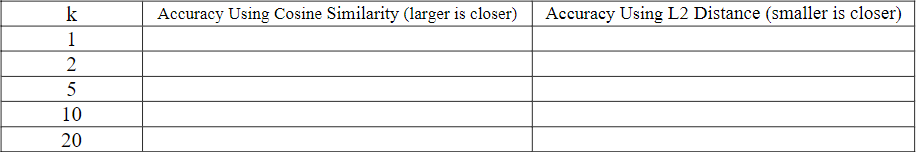
\includegraphics[width=\textwidth]{P2/table_task_1.png}

Since you need to choose three groups, you should have three tables. Note that cosine similarity is a similarity measure (the closer two vectors are, the larger the cosine similarity between them) while L2 distance (Euclidean distance) is a distance measure (the closer two vectors are, the smaller the L2 distance between them).
\end{problem}

%------------------------------------------------

\subsection*{Answer} For this assignment, we will use the GPT-2 model available on HuggingFace \cite{hf_canonical_model_maintainers_2022}. Moreover, we will make tables for \texttt{capital-common-countries}, 
\texttt{currency}, and \texttt{family} groups since they have the smallest sizes. As our method is relatively simple, we would not expect the accuracy to be high, but we believe the results should be better than chance.  Table \ref{tab: capital-common-countries} shows the result for group \texttt{capita-common-countries}.
\begin{table}[H]
\centering
\begin{tabular}{ccc}
\hline
\textbf{k} & \textbf{Accuracy Using Cosine Similarity} & \textbf{Accuracy Using L2 Distance} \\
\hline
1 & 0.061265 & 0.037549 \\
2 & 0.108696 & 0.075099 \\
5 & 0.250988 & 0.225296 \\
10 & 0.413043 & 0.446640 \\
20 & 0.877470 & 0.883399 \\
\hline
\end{tabular}
\caption{Results for group \texttt{capital-common-countries}}
\label{tab: capital-common-countries}
\end{table}

There are 23 candidate words, so getting it correct by chance is $k/23=0.043$, especially $1/23\sim 0.043$. Contrary to the prior belief, the result shows that the L2 results perform worse or are similar to random guesses. Table \ref{tab: currency} shows the results for the group
\texttt{currency}.

\begin{table}[H]
\centering
\begin{tabular}{ccc}
\hline
\textbf{k} & \textbf{Accuracy Using Cosine Similarity} & \textbf{Accuracy Using L2 Distance} \\
\hline
1 & 0.025404 & 0.031178 \\
2 & 0.060046 & 0.081986 \\
5 & 0.161663 & 0.195150 \\
10 & 0.352194 & 0.391455 \\
20 & 0.706697 & 0.742494 \\
\hline
\end{tabular}
\caption{Results for group \texttt{currency}}
\label{tab: currency}
\end{table}

There were 28 candidate words, so again, the random guesses will achieve the average accuracy of $k/28$. We can, again, see that the performance is worse or only marginally better than the random guess. Finally, Table \ref{tab: family} shows the result for the group \texttt{family}.

\begin{table}[H]
\centering
\begin{tabular}{ccc}
\hline
\textbf{k} & \textbf{Accuracy Using Cosine Similarity} & \textbf{Accuracy Using L2 Distance} \\
\hline
1 & 0.092885 & 0.173913 \\
2 & 0.162055 & 0.262846 \\
5 & 0.290514 & 0.450593 \\
10 & 0.456522 & 0.745059 \\
20 & 0.816206 & 0.966403 \\
\hline
\end{tabular}
\caption{Results for group \texttt{family}}
\label{tab: family}
\end{table}

There were also 23 candidate words here. We can observe remarkably better results here, but we do not see groundbreaking results. To summarise this task, we have observed disappointing results. This could be due to the fact that our method is very simple and also that the datasets we have chosen could be particularly bad for this task.
%----------------------------------------------------------------------------------------

\section*{Question 2}

\begin{problem}
First, we need to split the samples (the dataset is available from
https://www.cs.fsu.edu/liux/courses/deepRL/assignments/amazon\_reviews.csv) into a training set and a test
set. We will use 80\% of the samples for training and the remaining ones for testing. Then you need to use
BERT or GPT to create a representation for each of the reviews. After that, you need to train a classifier using
the samples in the train set and then use the trained classifier to classify the samples in the test set. Optionally,
you can finetune BERT or GPT for sentiment classification by adding a classifier to BERT or GPT and
finetune the entire model using the training set and evaluate on the test set. Since the dataset is relatively
small, you should not over finetune the model. Note that there are five different ratings, 1.0, 2.0, 3.0, 4.0, and
5.0.
\end{problem}

%------------------------------------------------

\subsection*{Answer}


\bibliographystyle{plain}
\bibliography{P2/P2}

\end{document}
